In this lecture, we see the first quantum algorithms that beat every classical algorithm in the
query model: Deutsch's algorithm and, using the \emph{phase flip} form of a query and the $n$-qubit
Hadamard (Walsh--Hadamard) transform, the Deutsch--Jozsa algorithm.

\section{Deutsch's Algorithm}

\begin{problem}[Deutsch's Problem]
    Given a function $f \colon \set{0,1} \to \set{0,1}$ as a black box, determine whether $f$ is
    \emph{constant} ($f(0) = f(1)$) or \emph{balanced} ($f(0) \neq f(1)$).
\end{problem}

Classically we need $2$ queries: after one query, say $f(0)$, both answers are still possible.
Quantumly, Deutsch's algorithm does it with $1$ query.

\subsection{The Quantum Query \texorpdfstring{$U_f$}{Uf}}

A quantum circuit is reversible, but $f$ need not be. We therefore convert $f$ into a reversible
\emph{quantum version} $U_f$, a controlled-$f$ gate like the CNOT gate of \cref{def:cnot-0915}
(\cref{fig:uf-0924}):
\[U_f \colon \ket{a}\ket{b} \longmapsto \ket{a}\ket{b \oplus f(a)}.\]
Applying $U_f$ twice gives back $\ket{a}\ket{b}$, so $U_f$ is reversible. One application of $U_f$
counts as one query to $f$.

\begin{figure}[ht]
    \centering
    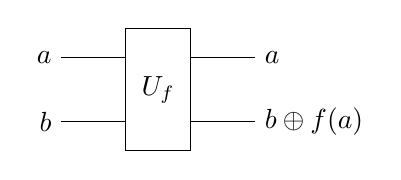
\begin{tikzpicture}[scale=0.82]
        \draw (0,1) -- (3,1);
        \draw (0,0) -- (3,0);
        \node[left] at (0,1) {$\ket{a}$};
        \node[left] at (0,0) {$\ket{b}$};
        \draw[fill=white] (1,-0.45) rectangle (2,1.45);
        \node at (1.5,0.5) {$U_f$};
        \node[right] at (3,1) {$\ket{a}$};
        \node[right] at (3,0) {$\ket{b \oplus f(a)}$};
    \end{tikzpicture}
    \caption{The quantum query $U_f$.}
    \label{fig:uf-0924}
\end{figure}

\subsection{The Circuit}

In Deutsch's algorithm (\cref{fig:deutsch-0924}) the qubits start in $\ket{0}$ and $\ket{1}$, go
through a Hadamard gate each, then through $U_f$, then through a Hadamard gate each, and are measured.

\begin{figure}[ht]
    \centering
    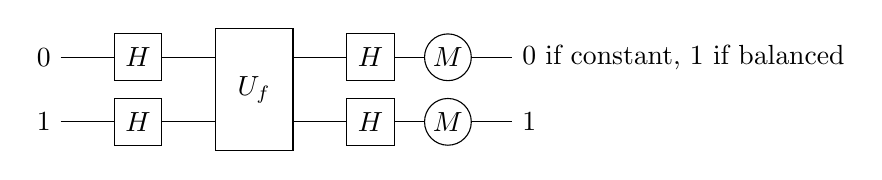
\begin{tikzpicture}[scale=0.82, 
            gate/.style={draw, fill=white, minimum size=6mm, inner sep=1pt},
            meter/.style={draw, circle, fill=white, inner sep=1.5pt},
        ]
        % wires
        \draw (0,1) -- (7,1);
        \draw (0,0) -- (7,0);
        \node[left] at (0,1) {$\ket{0}$};
        \node[left] at (0,0) {$\ket{1}$};
        % query
        \draw[fill=white] (2.4,-0.45) rectangle (3.6,1.45);
        \node at (3,0.5) {$U_f$};
        % Hadamard gates and measurements
        \foreach \y in {0,1} {
                \node[gate] at (1.2,\y) {$H$};
                \node[gate] at (4.8,\y) {$H$};
                \node[meter] at (6,\y) {$M$};
            }
        \node[right] at (7,1) {$\ket{0}$ if constant, $\ket{1}$ if balanced};
        \node[right] at (7,0) {$\ket{1}$};
    \end{tikzpicture}
    \caption{Deutsch's algorithm.}
    \label{fig:deutsch-0924}
\end{figure}

By \cref{eq:hadamard-0915}, for $a \in \set{0,1}$,
\begin{equation}\label{eq:hadamard-0924}
    H\ket{a} = \frac{1}{\sqrt{2}}\left(\ket{0} + (-1)^{a}\ket{1}\right)
    = \frac{1}{\sqrt{2}} \sum_{b \in \set{0,1}} (-1)^{ab} \ket{b}.
\end{equation}

\begin{exercise}\label{ex:hback-0924}
    Compute $H \, \frac{1}{\sqrt{2}}\left(\ket{0} + (-1)^{a}\ket{1}\right)$ for $a \in \set{0,1}$.
\end{exercise}

\begin{wsolution}
    By linearity and \cref{eq:hadamard-0924} for $H\ket{0}$ and $H\ket{1}$,
    \[H \, \tfrac{1}{\sqrt{2}}\left(\ket{0} + (-1)^{a}\ket{1}\right)
        = \tfrac{1}{2}\left(\ket{0} + \ket{1}\right) + \tfrac{(-1)^{a}}{2}\left(\ket{0} - \ket{1}\right)
        = \tfrac{1 + (-1)^{a}}{2}\ket{0} + \tfrac{1 - (-1)^{a}}{2}\ket{1}.\]
    For $a = 0$ this is $\ket{0}$ and for $a = 1$ it is $\ket{1}$, so the result is $\ket{a}$. This
    agrees with $H^2 = I$ (\cref{lem:hh-0915}).
\end{wsolution}

\begin{exercise}\label{ex:deutsch-0924}
    In the circuit of \cref{fig:deutsch-0924} the second qubit is measured as $\ket{1}$. What does the
    measurement of the first qubit give?
\end{exercise}

The answer is $\ket{0}$ if $f$ is constant and $\ket{1}$ if $f$ is balanced:

\begin{theorem}[Deutsch's Algorithm]\label{thm:deutsch-0924}
    The circuit of \cref{fig:deutsch-0924} makes one query to $f$, and measuring its first qubit gives
    $f(0) \oplus f(1)$ with probability $1$. Hence the outcome is $0$ if $f$ is constant and $1$ if $f$
    is balanced.
\end{theorem}

\begin{proof}
    After the first two Hadamard gates the state is (by \cref{eq:mixed-0915})
    $\ket{\psi_1} = H\ket{0} \otimes H\ket{1}
        = \frac{1}{2}\left(\ket{0} + \ket{1}\right)\left(\ket{0} - \ket{1}\right)$.
    For $c \in \set{0,1}$ we have
    $\ket{0 \oplus c} - \ket{1 \oplus c} = (-1)^{c}\left(\ket{0} - \ket{1}\right)$ (for $c = 1$ the two
    kets are swapped), so $U_f$ maps $\ket{a}\left(\ket{0} - \ket{1}\right)$ to
    $(-1)^{f(a)} \ket{a}\left(\ket{0} - \ket{1}\right)$ and, by linearity,
    \[\ket{\psi_2} = U_f \ket{\psi_1}
        = \frac{1}{\sqrt{2}}\left((-1)^{f(0)}\ket{0} + (-1)^{f(1)}\ket{1}\right)
        \otimes \frac{1}{\sqrt{2}}\left(\ket{0} - \ket{1}\right).\]
    Since $(-1)^{f(1)} = (-1)^{f(0)} (-1)^{f(0) \oplus f(1)}$, the first qubit is
    $(-1)^{f(0)} \frac{1}{\sqrt{2}}\left(\ket{0} + (-1)^{f(0) \oplus f(1)}\ket{1}\right)$, i.e., up to the
    sign $(-1)^{f(0)}$, the state of \cref{ex:hback-0924} with $a = f(0) \oplus f(1)$; the
    second qubit is $H\ket{1}$. So the last two Hadamard gates give
    $\ket{\psi_3} = (-1)^{f(0)} \ket{f(0) \oplus f(1)} \ket{1}$.
    The global phase $(-1)^{f(0)}$ does not affect the measurement: the first qubit gives
    $f(0) \oplus f(1)$ with probability $1$, and the second always gives $1$.
\end{proof}

\section{Phase Flip and the \texorpdfstring{$n$}{n}-Qubit Hadamard Transform}

If the second (target) qubit of $U_f$ is in the state
$\frac{1}{\sqrt{2}}\left(\ket{0} - \ket{1}\right)$, then, by the computation in the proof of
\cref{thm:deutsch-0924}, for every input $x$ (also for $x \in \set{0,1}^n$, where
$U_f \colon \ket{x}\ket{b} \mapsto \ket{x}\ket{b \oplus f(x)}$),
\[U_f \, \ket{x} \tfrac{1}{\sqrt{2}}(\ket{0} - \ket{1}) = (-1)^{f(x)} \, \ket{x} \tfrac{1}{\sqrt{2}}(\ket{0} - \ket{1}).\]
We drop the target qubit and write the query in the \emph{phase flip} form
\[U_f \colon \ket{x} \longmapsto (-1)^{f(x)} \ket{x}.\]
By linearity, $U_f$ maps $\sum_x \alpha_x \ket{x}$ to $\sum_x \alpha_x (-1)^{f(x)} \ket{x}$: one query
flips the sign of every $\ket{x}$ with $f(x) = 1$.

\subsection{The \texorpdfstring{$n$}{n}-Qubit Hadamard Transform}

To generalize Deutsch's algorithm to $n$ bits we apply the Hadamard gate to each of $n$ qubits.
Start with $n = 2$ and let $\ket{x} = \ket{x_1 x_2} = \ket{x_1}\ket{x_2}$. Using
\cref{eq:mixed-0915} and then \cref{eq:hadamard-0924} on each qubit,
\begin{align*}
    (H \otimes H)\ket{x}
     & = H\ket{x_1} \otimes H\ket{x_2}
    = \left(\frac{1}{\sqrt{2}} \sum_{y_1 \in \set{0,1}} (-1)^{x_1 y_1} \ket{y_1}\right)
    \left(\frac{1}{\sqrt{2}} \sum_{y_2 \in \set{0,1}} (-1)^{x_2 y_2} \ket{y_2}\right) \\
     & = \frac{1}{2} \sum_{y \in \set{0,1}^2} (-1)^{x_1 y_1 + x_2 y_2} \ket{y}
    = \frac{1}{2} \sum_{y \in \set{0,1}^2} (-1)^{x \cdot y} \ket{y},
\end{align*}
where $x \cdot y = x_1 y_1 \oplus x_2 y_2$, since only the parity of the exponent matters. For
example, $(H \otimes H)\ket{01} = \frac{1}{2}\left(\ket{00} - \ket{01} + \ket{10} - \ket{11}\right)$.
In general, for $x, y \in \set{0,1}^n$, the inner product of the bit strings modulo $2$ is
\[x \cdot y = x_1 y_1 \oplus x_2 y_2 \oplus \dots \oplus x_n y_n.\]

\begin{lemma}[Walsh--Hadamard Transform]\label{lem:wh-0924}
    The $n$-qubit Hadamard transform $H^{\otimes n} = H \otimes H \otimes \dots \otimes H$ (the
    \emph{Walsh--Hadamard transform}) acts on a basis state $\ket{x} = \ket{x_1 x_2 \cdots x_n}$ as
    \[H^{\otimes n} \ket{x} = \frac{1}{\sqrt{2^n}} \sum_{y \in \set{0,1}^n} (-1)^{x \cdot y} \ket{y}.\]
\end{lemma}

\begin{proof}
    By \cref{eq:mixed-0915} applied repeatedly, $H^{\otimes n} \ket{x} = H\ket{x_1} \otimes \dots \otimes H\ket{x_n}$,
    and by \cref{eq:hadamard-0924} the $\nth{i}$ factor is
    $\frac{1}{\sqrt{2}} \sum_{y_i \in \set{0,1}} (-1)^{x_i y_i} \ket{y_i}$. Multiplying out the $n$ sums,
    \[H^{\otimes n} \ket{x}
        = \frac{1}{\sqrt{2^n}} \sum_{y \in \set{0,1}^n} (-1)^{x_1 y_1 + \dots + x_n y_n} \ket{y},\]
    and $(-1)$ to the power $x_1 y_1 + \dots + x_n y_n$ only depends on its parity $x \cdot y$.
\end{proof}

For $x = 0^n = 00 \cdots 0$ we have $x \cdot y = 0$ for every $y$, so
$H^{\otimes n} \ket{00 \cdots 0} = \frac{1}{\sqrt{2^n}} \sum_{x \in \set{0,1}^n} \ket{x}$
is the uniform superposition of all $2^n$ bit strings.

\section{Deutsch--Jozsa Algorithm}

\begin{problem}[Deutsch--Jozsa Problem]
    Given $f \colon \set{0,1}^n \to \set{0,1}$ as a black box, with the \emph{promise} that $f$ is
    either constant or balanced (i.e., $f(x) = 0$ for exactly half of the $2^n$ inputs), determine
    which is the case.
\end{problem}

This is Deutsch's problem on $n$ bits. It is a \emph{promise problem}: we are told in advance that $f$
is one of the two kinds. Let $N = 2^n$ be the number of inputs.

\subsection{Classical Query Complexity}

\emph{Deterministic:} in the worst case $2^{n-1} + 1 = N/2 + 1$ queries are needed, since after $N/2$
equal values $f$ may still be either constant or balanced. The same holds for a randomized algorithm
that has to succeed with probability $1$.

\emph{Randomized (Monte Carlo):} query $f$ on $\alpha$ independent uniformly random inputs and output
``balanced'' if two answers differ, ``constant'' otherwise. If $f$ is constant, we are always right. If
$f$ is balanced, every answer is $0$ or $1$ with probability $\sfrac{1}{2}$ each, so all $\alpha$
answers agree, and we fail, with probability
$2 \cdot (\sfrac{1}{2})^{\alpha} = (\sfrac{1}{2})^{\alpha - 1}$. A constant number of queries gives a
constant error probability, and $\alpha = \bigO{\log N}$ queries give error probability $\sfrac{1}{N}$.

\emph{Quantum:} the Deutsch--Jozsa algorithm needs $1$ query (and $n$ measurements) and makes no error.

\subsection{The Algorithm}

The circuit (\cref{fig:dj-0924}) is Deutsch's circuit with $n$ input qubits: $n$ qubits in $\ket{0}$
and one qubit in $\ket{1}$ go through Hadamard gates and then $U_f$ (one query); then all the
qubits go through Hadamard gates again and are measured.

\begin{figure}[ht]
    \centering
    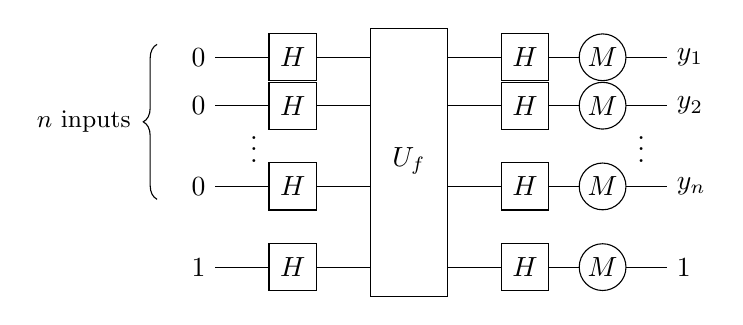
\begin{tikzpicture}[scale=0.82, 
            gate/.style={draw, fill=white, minimum size=6mm, inner sep=1pt},
            meter/.style={draw, circle, fill=white, inner sep=1.5pt},
        ]
        % wires: inputs y_1, y_2, ..., y_n, then the extra qubit
        \foreach \y in {3,2.25,1,-0.25} {\draw (0,\y) -- (7,\y);}
        \foreach \y in {3,2.25,1} {\node[left] at (0,\y) {$\ket{0}$};}
        \node[left] at (0,-0.25) {$\ket{1}$};
        \node at (0.6,1.7) {$\vdots$};
        \node at (6.6,1.7) {$\vdots$};
        % query
        \draw[fill=white] (2.4,-0.7) rectangle (3.6,3.45);
        \node at (3,1.4) {$U_f$};
        % Hadamard gates
        \foreach \y in {3,2.25,1,-0.25} {
                \node[gate] at (1.2,\y) {$H$};
                \node[gate] at (4.8,\y) {$H$};
                \node[meter] at (6,\y) {$M$};
            }
        % outputs
        \node[right] at (7,3) {$y_1$};
        \node[right] at (7,2.25) {$y_2$};
        \node[right] at (7,1) {$y_n$};
        \node[right] at (7,-0.25) {$\ket{1}$};
        % the n input qubits
        \draw[decorate, decoration={brace, amplitude=5pt}] (-0.9,0.8) -- (-0.9,3.2)
        node[midway, left=6pt] {\small $n$ inputs};
    \end{tikzpicture}
    \caption{The Deutsch--Jozsa algorithm. The last qubit always gives $1$.}
    \label{fig:dj-0924}
\end{figure}

\begin{exercise}\label{ex:dj-0924}
    The state of the $n$ input qubits before the measurement is
    $\frac{1}{2^n} \sum_{y} \sum_{x} (-1)^{f(x) + x \cdot y} \ket{y}$. What do the measurements give if
    $f$ is constant, and what if $f$ is balanced?
\end{exercise}

\begin{theorem}[Deutsch--Jozsa Algorithm]\label{thm:dj-0924}
    In the circuit of \cref{fig:dj-0924}, measuring the $n$ input qubits gives $y = 0^n$ with
    probability $1$ if $f$ is constant, and with probability $0$ if $f$ is balanced. Hence, if any
    of these $n$ measurements gives $1$, then $f$ is balanced; otherwise $f$ is constant.
\end{theorem}

\begin{proof}
    We use the phase flip form of $U_f$: the last qubit is
    $\frac{1}{\sqrt{2}}(\ket{0} - \ket{1}) = H\ket{1}$ before and after the query, so its second
    Hadamard gate gives $\ket{1}$, and we drop it. The first layer of Hadamard gates maps the input register
    $\ket{00 \cdots 0}$ to $\frac{1}{\sqrt{2^n}} \sum_{x} \ket{x}$, and the query flips the sign of
    every $\ket{x}$ with $f(x) = 1$. After the second layer of Hadamard gates, by \cref{lem:wh-0924},
    the state is
    \[\frac{1}{\sqrt{2^n}} \sum_{x \in \set{0,1}^n} (-1)^{f(x)} H^{\otimes n} \ket{x}
        = \frac{1}{2^n} \sum_{y \in \set{0,1}^n} \sum_{x \in \set{0,1}^n} (-1)^{f(x) + x \cdot y} \ket{y}.\]
    Since $x \cdot 0^n = 0$ for every $x$, the amplitude of $\ket{0^n}$ is
    $\frac{1}{2^n} \sum_{x} (-1)^{f(x)}$. If $f$ is constant, all $2^n$ terms are equal and the
    amplitude is $\pm 1$; the amplitudes squared sum to $1$, so all others are $0$ and the measurement
    gives $0^n$ with probability $1$. If $f$ is balanced, half the terms are $+1$ and half are $-1$, so
    the amplitude is $0$: the measurement gives $0^n$ with probability $0$, i.e., at least one of the
    $n$ measurements gives $1$.
\end{proof}
